\section{推論の高速化}
\label{sec_speed}
\subsection{プレフィックスの共有}
\ref{sec_vlm}章の分類器は，ボケ1件ごとに，お題画像のトークンとお題の文を含む約300トークンを計算する．
しかし，同じお題のボケ（平均約14件）では，入力の「ボケ：「」までの部分（プレフィックス）が共通である．
そこで，図\ref{fig_prefix}のように計算を分けた．

\begin{figure}[t]
    \centering
    \begin{tikzpicture}[font=\scriptsize, node distance=3mm,
        box/.style={draw, rounded corners=2pt, minimum height=5mm, align=center, inner sep=2pt}]
        \node[box, fill=gray!15, minimum width=34mm] (pre) {お題画像＋お題の文（プレフィックス）\\ 約250〜300トークン，お題ごとに1回};
        \node[box, below=4mm of pre, minimum width=34mm] (kv) {KV キャッシュ};
        \node[box, below left=5mm and -12mm of kv, minimum width=14mm] (s1) {ボケ1};
        \node[box, right=2mm of s1, minimum width=14mm] (s2) {ボケ2};
        \node[right=1mm of s2] (dots) {$\cdots$};
        \node[box, right=1mm of dots, minimum width=14mm] (sn) {ボケ $ n $};
        \node[box, below=4mm of s2, minimum width=50mm] (head) {最後のトークンの隠れ状態 $\rightarrow$ (\ref{eq_heads})};
        \draw[-{Stealth}] (pre) -- (kv);
        \draw[-{Stealth}] (kv) -- (s1);
        \draw[-{Stealth}] (kv) -- (s2);
        \draw[-{Stealth}] (kv) -- (sn);
        \draw[-{Stealth}] (s1) -- (head);
        \draw[-{Stealth}] (s2) -- (head);
        \draw[-{Stealth}] (sn) -- (head);
    \end{tikzpicture}
    \caption{プレフィックスの共有による推論．お題ごとにプレフィックスを1回計算して KV キャッシュを作り，ボケの数だけ複製して，ボケの文と閉じ括弧以降（約20〜60トークン）だけを計算する．}
    \label{fig_prefix}
\end{figure}

お題 $ g $ のボケの数を $ n_g $，プレフィックスの長さを $ L_{\rm p} $，ボケ $ i $ の部分の長さを $ L_{i} $ とすると，計算するトークン数は(\ref{eq_tokens})のように減る．

\begin{equation}
    \sum_{g} \sum_{i=1}^{n_g} ( L_{\rm p} + L_{i} ) \; \rightarrow \; \sum_{g} \left( L_{\rm p} + \sum_{i=1}^{n_g} L_{i} \right)
    \label{eq_tokens}
\end{equation}

\noindent
例えば $ n_g = 14 $，$ L_{\rm p} = 270 $，$ L_{i} = 40 $ とすると，計算するトークン数は約1/5になる．
InternVL3.5 は画像のトークン数が一定であるため，プレフィックスの長さが同じお題をまとめて計算した．
Qwen3-VL は画像ごとにトークン数が異なり，位置が3次元の回転位置埋め込みであるため，プレフィックスを左詰めでまとめて計算し，ボケの部分の位置はプレフィックスの最大の位置の次から続けた．
プレフィックスとボケの部分は別々にトークン化するため，境界のトークン化が通常の推論とわずかに異なる場合がある．

\subsection{結果}
検証データ620件で通常の推論と比べると，判定の一致は InternVL3.5-2B で99.7\%，Qwen3-VL-4B で99.8\%，画像外の知識の確率の差の平均は0.003であった．
速度は，データベースから無作為に選んだ600件のお題の全てのボケ（8,664件，1お題あたり14.4件）を，画像の読み込みと前処理を含めて処理して測った．
GPU は RTX PRO 6000（96GB）1枚，前処理は8プロセスである．
図\ref{fig_speed}に結果を示す．

\begin{figure}[t]
    \centering
    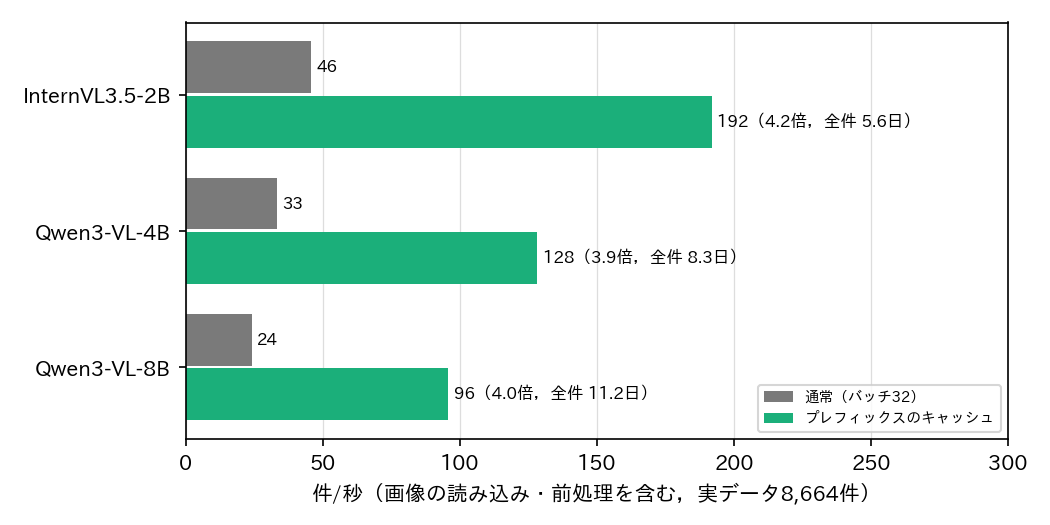
\includegraphics[width=\linewidth]{figures/fig_speed.png}
    \caption{通常の推論（バッチ32）とプレフィックスの共有による推論の1秒あたりの件数．括弧内は倍率と，約9,250万件の推定処理日数である．}
    \label{fig_speed}
\end{figure}

プレフィックスの共有により，InternVL3.5-2B は46件/秒から192件/秒，Qwen3-VL-4B は33件/秒から128件/秒，Qwen3-VL-8B は24件/秒から96件/秒となり，いずれも約4倍に高速化した．
全件の推定処理時間は，Qwen3-VL-4B で約32日から約8.3日，Qwen3-VL-8B で約11日となった．
一度にまとめるボケを1,024件に増やすと GPU のメモリの圧迫で遅くなり，256〜512件が最適であった．
前処理のプロセスを16に増やしても速くならなかったため，GPU の計算が律速である．

表\ref{tab_time}に，本稿で扱った主な方法で全件を処理する場合の推定時間をまとめる．
VLM の教師を全件に適用するには数か月から1年近くを要し，現実的ではない．
文の生徒は数時間で処理できるが，画像外の知識の精度が低い．
プレフィックスを共有した小さな VLM は，精度と処理時間の両方で実用的な範囲にある．

\begin{table}[t]
    \centering
    \caption{約9,250万件の処理時間の見積もり（単一の GPU）．F1 は最終評価用（合意ラベル）．}
    \label{tab_time}
    \footnotesize
    \setlength{\tabcolsep}{2.5pt}
    \begin{tabular}{@{}lcccr@{}}
        \toprule
        方法 & 件/秒 & 6区分 & 画像外 & 全件 \\
        \midrule
        教師 32B（one\_kt\_cap） & 3.9 & 0.56 & 0.67 & 約270日 \\
        文の生徒 & --- & 0.61 & 0.60 & 数時間 \\
        Qwen3-VL-4B（通常） & 33 & 0.71 & 0.69 & 約32日 \\
        InternVL3.5-2B（共有） & 192 & 0.71 & 0.64 & 約5.6日 \\
        Qwen3-VL-4B（共有） & 128 & 0.71 & 0.69 & 約8.3日 \\
        Qwen3-VL-8B（共有） & 96 & 0.74 & 0.68 & 約11日 \\
        Qwen3-VL-4B＋8B（共有） & 55 & 0.71 & 0.70 & 約19日 \\
        \bottomrule
    \end{tabular}
\end{table}
